%% abtex2-modelo-trabalho-academico.tex, v-1.9.2 laurocesar
%% Copyright 2012-2014 by abnTeX2 group at http://abntex2.googlecode.com/ 
%%
%% This work may be distributed and/or modified under the
%% conditions of the LaTeX Project Public License, either version 1.3
%% of this license or (at your option) any later version.
%% The latest version of this license is in
%%   http://www.latex-project.org/lppl.txt
%% and version 1.3 or later is part of all distributions of LaTeX
%% version 2005/12/01 or later.
%%
%% This work has the LPPL maintenance status `maintained'.
%% 
%% The Current Maintainer of this work is the abnTeX2 team, led
%% by Lauro César Araujo. Further information are available on 
%% http://abntex2.googlecode.com/
%%
%% This work consists of the files abntex2-modelo-trabalho-academico.tex,
%% abntex2-modelo-include-comandos and abntex2-modelo-references.bib
%%

% ------------------------------------------------------------------------
% ------------------------------------------------------------------------
% abnTeX2: Modelo de Trabalho Academico (tese de doutorado, dissertacao de
% mestrado e trabalhos monograficos em geral) em conformidade com 
% ABNT NBR 14724:2011: Informacao e documentacao - Trabalhos academicos -
% Apresentacao
% ------------------------------------------------------------------------
% ------------------------------------------------------------------------

%-------------------------------------------------------------------------
% Modelo adaptado especificamente para o contexto do PPgSI-EACH-USP por 
% Marcelo Fantinato, com auxílio dos Professores Norton T. Roman, Helton
% H. Bíscaro e Sarajane M. Peres, em 2015, com muitos agradecimentos aos 
% criadores da classe e do modelo base.
%
% 20/06/2017: inclusão de "lista de quadros" com base no especificado em:
% https://github.com/abntex/abntex2/wiki/HowToCriarNovoAmbienteListing,
% de autoria de "Eduardo de Santana Medeiros Alexandre".
%
%-------------------------------------------------------------------------

\documentclass[
	% -- opções da classe memoir --
	12pt,				% tamanho da fonte
	% openright,			% capítulos começam em pág ímpar (insere página vazia caso preciso)
	oneside,			% para impressão apenas no anverso (apenas frente). Oposto a twoside
	a4paper,			% tamanho do papel. 
	% -- opções da classe abntex2 --
	%chapter=TITLE,		% títulos de capítulos convertidos em letras maiúsculas
	%section=TITLE,		% títulos de seções convertidos em letras maiúsculas
	%subsection=TITLE,	% títulos de subseções convertidos em letras maiúsculas
	%subsubsection=TITLE,% títulos de subsubseções convertidos em letras maiúsculas
	% -- opções do pacote babel --
	english,			% idioma adicional para hifenização
	%french,				% idioma adicional para hifenização
	%spanish,			% idioma adicional para hifenização
	brazil				% o último idioma é o principal do documento
	]{abntex2unama}

% ---
% Pacotes básicos 
% ---
\usepackage{lmodern}			% Usa a fonte Latin Modern			
\usepackage[T1]{fontenc}		% Selecao de codigos de fonte.
\usepackage[utf8]{inputenc}		% Codificacao do documento (conversão automática dos acentos)
\usepackage{lastpage}			% Usado pela Ficha catalográfica
\usepackage{indentfirst}		% Indenta o primeiro parágrafo de cada seção.
\usepackage{color}				% Controle das cores
\usepackage{graphicx}			% Inclusão de gráficos
\usepackage{microtype} 			% para melhorias de justificação
\usepackage{pdfpages}     %para incluir pdf
\usepackage{algorithm}			%para ilustrações do tipo algoritmo
\usepackage{mdwlist}			%para itens com espaço padrão da abnt
\usepackage[noend]{algpseudocode}			%para ilustrações do tipo algoritmo
		
% ---
% Pacotes adicionais, usados apenas no âmbito do Modelo Canônico do abnteX2
% ---
\usepackage{lipsum}				% para geração de dummy text
% ---

% ---
% Pacotes de citações
% ---
\usepackage{hyperref}
\usepackage[brazilian,hyperpageref]{backref}	 % Paginas com as citações na bibl
\usepackage[alf,abnt-etal-list=0,abnt-etal-text=it]{abntex2cite}	% Citações padrão ABNT

% --- 
% CONFIGURAÇÕES DE PACOTES
% --- 

% ---
% Configurações do pacote backref
% Usado sem a opção hyperpageref de backref
\renewcommand{\backrefpagesname}{Citado na(s) página(s):~}
% Texto padrão antes do número das páginas
\renewcommand{\backref}{}
% Define os textos da citação
\renewcommand*{\backrefalt}[4]{
	\ifcase #1 %
		Nenhuma citação no texto.%
	\or
		Citado na página #2.%
	\else
		Citado #1 vezes nas páginas #2.%
	\fi}%
% ---

% ---
% Informações de dados para CAPA e FOLHA DE ROSTO
% ---

%-------------------------------------------------------------------------
% Comentário adicional do PPgSI - Informações sobre o ``instituicao'':
%
% Não mexer. Deixar exatamente como está.
%
%-------------------------------------------------------------------------
\instituicao{
	UNIVERSIDADE DA AMAZÔNIA
	\par
	CURSO DE BACHARELADO EM CIÊNCIA DA COMPUTAÇÃO
	\par
	DISCIPLINA DE INFRAESTRUTURA DE DATACENTERS
	}

%-------------------------------------------------------------------------
% Comentário adicional do PPgSI - Informações sobre o ``título'':
%
% Em maiúscula apenas a primeira letra da sentença (do título), exceto 
% nomes próprios, geográficos, institucionais ou Programas ou Projetos ou 
% siglas, os quais podem ter letras em maiúscula também.
%
% O subtítulo do trabalho é opcional.
% Sem ponto final.
%
% Atenção: o título da Dissertação/Tese na versão corrigida não pode mudar. 
% Ele deve ser idêntico ao da versão original.
%
%-------------------------------------------------------------------------
\titulo{Relatório Técnico: Avaliação de Viabilidade e Proposta de Projeto, Construção e Operação de Datacenter Próprio para Autopass/Tecsomobi}

%-------------------------------------------------------------------------
% Comentário adicional do PPgSI - Informações sobre o ``autor'':
%
% Todas as letras em maiúsculas.
% Nome completo.
% Sem ponto final.
% Para adicionar mais de um autor, basta acrescentar \\ entre os autores.
%-------------------------------------------------------------------------
\autor{DANIEL BAHIA PINHEIRO CALLIARI}

%-------------------------------------------------------------------------
% Comentário adicional do PPgSI - Informações sobre o ``local'':
%
% Não incluir o ``estado''.
% Sem ponto final.
%-------------------------------------------------------------------------
\local{Belém}

%-------------------------------------------------------------------------
% Comentário adicional do PPgSI - Informações sobre a ``data'':
%
% Colocar o ano do depósito (ou seja, o ano da entrega) da respectiva 
% versão, seja ela a versão original (para a defesa) seja ela a versão 
% corrigida (depois da aprovação na defesa). 
%
% Atenção: Se a versão original for depositada no final do ano e a versão 
% corrigida for entregue no ano seguinte, o ano precisa ser atualizado no 
% caso da versão corrigida. 
% Cuidado, pois o ano da ``capa externa'' também precisa ser atualizado 
% nesse caso.
%
% Não incluir o dia, nem o mês.
% Sem ponto final.
%-------------------------------------------------------------------------
\data{2025}

%-------------------------------------------------------------------------
% Comentário adicional do PPgSI - Informações sobre o ``Orientador'':
%
% Se for uma professora, trocar por ``Profa. Dra.''
% Nome completo.
% Sem ponto final.
%-------------------------------------------------------------------------
\orientador{Prof. Rodrigo Marques}

%-------------------------------------------------------------------------
% Comentário adicional do PPgSI - Informações sobre o ``Coorientador'':
%
% Opcional. Incluir apenas se houver co-orientador formal, de acordo com o 
% Regulamento do Programa.
%
% Se for uma professora, trocar por ``Profa. Dra.''
% Nome completo.
% Sem ponto final.
%-------------------------------------------------------------------------
% \coorientador{Prof. Dr. Fulano de Tal} % Removido ou ajustar se necessário

\tipotrabalho{Relatório Técnico} % Alterado

\preambulo{
%-------------------------------------------------------------------------
% Comentário adicional do PPgSI - Informações sobre o texto ``Versão 
% original'':
%
% Não usar para Qualificação.
% Não usar para versão corrigida de Dissertação/Tese.
%
%-------------------------------------------------------------------------
Versão original \newline \newline \newline
%-------------------------------------------------------------------------
% Comentário adicional do PPgSI - Informações sobre o ``texto principal do
% preambulo'':
%
% Para Doutorado, trocar por: Tese apresentada à Escola de Artes, Ciências e Humanidades da Universidade de São Paulo para obtenção do título de Doutor (ou Doutora) em Ciências pelo Programa de Pós-graduação em Sistemas de Informação. 
%
% Para Qualificação, trocar por: Projeto de pesquisa para exame de qualificação apresentado à Escola de Artes, Ciências e Humanidades da Universidade de São Paulo como parte dos requisitos para obtenção do título de Mestre (ou Doutor ou Doutora) em Ciências pelo Programa de Pós-graduação em Sistemas de Informação.
%
%-------------------------------------------------------------------------
Relatório técnico apresentado à Universidade da Amazõnia referente à Segunda Avaliação da disciplina de Infraestrutura de Datacenters do curso de Bacharelado em Ciência da Computação.
%
\newline \newline Área de concentração: Infraestrutura de Datacenters
%-------------------------------------------------------------------------
% Comentário adicional do PPgSI - Informações sobre o texto da ``Versão 
% corrigida'':
%
% Não usar para Qualificação.
% Não usar para versão original de Dissertação/Tese.
% 
% Substituir ``xx de xxxxxxxxxxxxxxx de xxxx'' pela ``data da defesa''.
%
%-------------------------------------------------------------------------
% \newline \newline \newline Versão corrigida contendo as alterações solicitadas pela comissão julgadora em xx de xxxxxxxxxxxxxxx de xxxx. A versão original encontra-se em acervo reservado na Biblioteca da EACH-USP e na Biblioteca Digital de Teses e Dissertações da USP (BDTD), de acordo com a Resolução CoPGr 6018, de 13 de outubro de 2011.
}
% ---


% ---
% Configurações de aparência do PDF final

% alterando o aspecto da cor azul
\definecolor{blue}{RGB}{41,5,195}

% informações do PDF
\makeatletter
\hypersetup{
     	%pagebackref=true,
		pdftitle={\@title}, 
		pdfauthor={\@author},
    	pdfsubject={\imprimirpreambulo},
	    pdfcreator={laTeX com abnTeX2 adaptado para a UNAMA/ALC},
		pdfkeywords={abnt}{latex}{abntex}{abntex2unama}{trabalho acadêmico}{unama}, 
		colorlinks=true,       		% false: boxed links; true: colored links
    	linkcolor=blue,          	% color of internal links
    	citecolor=blue,        		% color of links to bibliography
    	filecolor=magenta,      		% color of file links
		urlcolor=blue,
		bookmarksdepth=4
}
\makeatother
% --- 

% --- 
% Espaçamentos entre linhas e parágrafos 
% --- 

% O tamanho do parágrafo é dado por:
\setlength{\parindent}{1.25cm}

% Controle do espaçamento entre um parágrafo e outro:
\setlength{\parskip}{0cm}  % tente também \onelineskip
\renewcommand{\baselinestretch}{1.5}

% ---
% compila o indice
% ---
\makeindex
% ---

	% Controlar linhas orfas e viuvas
  \clubpenalty10000
  \widowpenalty10000
  \displaywidowpenalty10000

% ----
% Início do documento
% ----
\begin{document}

% Retira espaço extra obsoleto entre as frases.
\frenchspacing

% ----------------------------------------------------------
% ELEMENTOS PRÉ-TEXTUAIS
% ----------------------------------------------------------
% \pretextual

% ---
% Capa
% ---
%-------------------------------------------------------------------------
% Comentário adicional do PPgSI - Informações sobre a ``capa'':
%
% Esta é a ``capa'' principal/oficial do trabalho, a ser impressa apenas 
% para os casos de encadernação simples (ou seja, em ``espiral'' com 
% plástico na frente).
% 
% Não imprimir esta ``capa'' quando houver ``capa dura'' ou ``capa brochura'' 
% em que estas mesmas informações já estão presentes nela.
%
%-------------------------------------------------------------------------
\imprimircapa
% ---

% ---
% inserir o sumario
% ---
\pdfbookmark[0]{\contentsname}{toc}
\tableofcontents*
\cleardoublepage
% ---



% ----------------------------------------------------------
% ELEMENTOS TEXTUAIS
% ----------------------------------------------------------
\textual



%-------------------------------------------------------------------------
% Comentário adicional do PPgSI - Informações sobre ``títulos de seções''
% 
% Para todos os títulos (seções, subseções, tabelas, ilustrações, etc.):
%
% Em maiúscula apenas a primeira letra da sentença (do título), exceto 
% nomes próprios, geográficos, institucionais ou Programas ou Projetos ou
% siglas, os quais podem ter letras em maiúscula também.
%
\chapter{Introdução}
Este relatório tem como objetivo principal avaliar a viabilidade técnica e financeira da implementação de um datacenter próprio para a Autopass/Tecsomobi, além de propor um plano de projeto, construção e operação. Atualmente, a empresa utiliza uma vasta gama de serviços da Amazon Web Services (AWS), incluindo S3 para armazenamento, EC2 para capacidade computacional, Lambda para funções serverless, RDS para bancos de dados e VPC para redes privadas virtuais, entre outros \cite{cloud_infrastructure}. Esses serviços suportam operações críticas como VPN para funcionários, armazenamento de bancos de dados, e hospedagem de APIs e aplicações web (sites React) em ambientes de homologação e produção \cite{software_defined}.

A infraestrutura em nuvem está distribuída geograficamente para atender às operações em São Paulo, Belém do Pará, Rio de Janeiro, Votorantim, Sant'Ana do Livramento, Araras, Itapecerica da Serra, Barretos, Bertioga, Guarujá, etc. O custo diário com os serviços AWS é de aproximadamente US\$ 2.000, totalizando cerca de US\$ 60.000 mensais ou US\$ 720.000 anuais. Diante desse cenário, a construção de um datacenter próprio surge como uma alternativa estratégica para otimizar custos a longo prazo, aumentar o controle sobre a infraestrutura e personalizar a segurança e a performance de acordo com as necessidades específicas da Autopass/Tecsomobi \cite{datacenter_monitoring} \cite{reliability_engineering}. Este relatório detalhará os aspectos envolvidos nessa transição, desde a análise da arquitetura atual \cite{design_principles} até as recomendações finais para implementação de um sistema eficiente de gestão integrada da infraestrutura \cite{dcim_systems}.

\chapter{Arquitetura Atual e Análise de Custos AWS}
\section{Serviços AWS em Uso}
A Autopass/Tecsomobi utiliza um portfólio diversificado de serviços AWS para suportar suas operações \cite{cloud_infrastructure}. Os principais serviços incluem:
\begin{itemize}
	\item \textbf{Amazon S3 (Simple Storage Service):} Utilizado para armazenamento de objetos, como dados de biometria facial, boletos digitais, documentos pessoais digitalizados, backups de bancos de dados, arquivos de log e ativos de aplicações web \cite{datacenter_security}. Este serviço é crítico para o armazenamento de longo prazo dos dados de identificação dos usuários e documentos relacionados a transações.
	\item \textbf{AWS Lambda:} Permite a execução de código sem a necessidade de provisionar ou gerenciar servidores \cite{containerization}. É utilizado principalmente para validação de transações e processamento de recargas nas mídias físicas, permitindo escalabilidade automática conforme o volume de operações.
	\item \textbf{Amazon RDS (Relational Database Service):} Oferece bancos de dados relacionais gerenciados, como PostgreSQL, MySQL ou SQL Server, utilizados para armazenar dados transacionais das aplicações \cite{capacity_planning}.
	\item \textbf{Amazon VPC (Virtual Private Cloud):} Permite o provisionamento de uma seção logicamente isolada da Nuvem AWS, onde os recursos da AWS podem ser executados em uma rede virtual definida pela empresa \cite{network_fabric}. Utilizada para criar redes seguras para os ambientes de homologação e produção.
	\item \textbf{AWS VPN (Virtual Private Network):} Soluções como AWS Site-to-Site VPN e AWS Client VPN são utilizadas para prover acesso seguro à rede da empresa para funcionários remotos e para conectar escritórios e filiais à infraestrutura na nuvem \cite{datacenter_networking}.
	\item \textbf{Outros Serviços:} Adicionalmente, podem estar em uso serviços como Elastic Load Balancing (ELB), Amazon Route 53 (DNS), AWS IAM (Identity and Access Management), Amazon CloudWatch (monitoramento), entre outros \cite{software_defined}.
\end{itemize}

\section{Distribuição Geográfica dos Ambientes}
Os ambientes da Autopass/Tecsomobi estão distribuídos para atender às necessidades de negócio e garantir a proximidade dos usuários e serviços \cite{modular_datacenters}. A distribuição inclui:
\begin{itemize}
	\item \textbf{São Paulo (Capital e Interiores):} Concentra a maior parte da infraestrutura de produção e homologação, devido à importância estratégica e volume de operações. Possui equipe técnica dedicada in loco \cite{hyperscale_datacenters}.
	\item \textbf{Belém:} Suporta operações regionais com equipe técnica local, funcionando como um hub secundário para atender usuários da região Norte \cite{edge_computing}.
	\item \textbf{Rio de Janeiro:} Possui infraestrutura na nuvem para suportar as operações na região, sem equipe técnica in loco.
	\item \textbf{Demais Cidades (Vitória, Votorantim, Itapecerica da Serra, Guarujá, etc.):} Acessam recursos e serviços exclusivamente via nuvem, sendo gerenciados remotamente pelas equipes de São Paulo e Belém \cite{datacenter_monitoring}.
\end{itemize}
Cada localidade pode possuir ambientes de homologação (desenvolvimento, testes, Q\&A) e produção, com diferentes níveis de criticidade e requisitos de disponibilidade \cite{reliability_engineering}.

\section{Análise de Custos}
O custo atual com serviços AWS é um fator motivador para a avaliação de um datacenter próprio \cite{dcim_evolution}.
\begin{itemize}
	\item \textbf{Custo Diário:} Aproximadamente US\$ 2.000.
	\item \textbf{Custo Mensal Estimado:} US\$ 2.000/dia * 30 dias = US\$ 60.000.
	\item \textbf{Custo Anual Estimado:} US\$ 60.000/mês * 12 meses = US\$ 720.000.
\end{itemize}
Estes custos podem variar conforme o uso de recursos, tráfego de dados, tipos de instância e serviços adicionais contratados. Uma análise detalhada dos relatórios de faturamento da AWS (AWS Cost Explorer, faturas detalhadas) é fundamental para identificar os principais centros de custo \cite{capacity_planning}.

\section{Pontos Fortes e Limitações do Modelo de Nuvem (AWS)}
\subsection{Pontos Fortes}
\begin{itemize}
	\item \textbf{Escalabilidade e Elasticidade:} Capacidade de aumentar ou diminuir recursos rapidamente conforme a demanda \cite{cloud_infrastructure}.
	\item \textbf{Modelo de Pagamento Conforme o Uso (Pay-as-you-go):} Evita grandes investimentos iniciais em hardware \cite{datacenter_automation}.
	\item \textbf{Ampla Gama de Serviços Gerenciados:} Reduz a carga de gerenciamento de infraestrutura em diversas áreas (bancos de dados, redes, etc.) \cite{ai_automation}.
	\item \textbf{Alcance Global e Alta Disponibilidade:} Datacenters distribuídos globalmente com opções de redundância e alta disponibilidade \cite{disaster_recovery}.
	\item \textbf{Inovação Contínua:} Acesso rápido a novas tecnologias e serviços \cite{software_defined}.
\end{itemize}

\subsection{Limitações}
\begin{itemize}
	\item \textbf{Custos Elevados em Escala:} Para cargas de trabalho estáveis e de grande volume, os custos operacionais podem se tornar significativos e superar o TCO de uma infraestrutura própria a longo prazo \cite{dcim_systems}.
	\item \textbf{Menor Controle e Personalização:} Menor flexibilidade para customizações profundas de hardware e otimizações específicas de rede em comparação com um datacenter próprio \cite{design_principles}.
	\item \textbf{Dependência do Provedor (Vendor Lock-in):} Dificuldade e custo para migrar cargas de trabalho para outros provedores ou para uma infraestrutura on-premise \cite{containerization}.
	\item \textbf{Previsibilidade de Custos:} Embora o modelo seja pay-as-you-go, picos inesperados de uso ou tráfego de dados podem levar a custos não previstos \cite{power_distribution}.
	\item \textbf{Questões de Conformidade e Soberania de Dados:} Para alguns setores ou regulamentações, manter dados em infraestrutura de terceiros, mesmo que segura, pode apresentar desafios \cite{datacenter_security}.
\end{itemize}

\chapter{Requisitos e Escopo do Datacenter}
\section{Requisitos de Capacidade}
O dimensionamento da capacidade do datacenter deve considerar o consumo atual de recursos na AWS e prever o crescimento futuro \cite{capacity_planning}.
\begin{itemize}
	\item \textbf{CPU (Unidades de Processamento Central):} Análise do consumo total de vCPUs nas instâncias EC2, RDS e outras cargas de trabalho. Considerar a utilização média e de pico \cite{hyperscale_datacenters}.
	\item \textbf{RAM (Memória de Acesso Aleatório):} Levantamento da memória total alocada e utilizada pelos serviços atuais.
	\item \textbf{Armazenamento:} Capacidade total de armazenamento em S3, EBS (Elastic Block Store), RDS e outros. Definir tiers de armazenamento (SSD de alta performance, discos SAS/SATA para capacidade) e IOPS (operações de entrada/saída por segundo) necessários \cite{dcim_systems}.
	\item \textbf{I/O de Rede (Entrada/Saída):} Largura de banda de rede interna e externa (internet) necessária para suportar as aplicações, APIs, VPNs e tráfego de usuários \cite{network_fabric}.
	\item \textbf{Banda de Internet:} Capacidade de links de internet dedicados, considerando redundância \cite{datacenter_networking}.
	\item \textbf{Previsão de Crescimento:} Estimar o crescimento da demanda por recursos nos próximos 3, 5 e 10 anos \cite{design_principles}.
\end{itemize}
Será necessário realizar um inventário detalhado dos recursos AWS para quantificar esses requisitos.

\section{SLA (Service Level Agreement) Desejado}
Definir os níveis de serviço esperados para os diferentes ambientes \cite{reliability_engineering}:
\begin{itemize}
	\item \textbf{Ambientes de Produção:} Requerem alta disponibilidade, por exemplo, 99,982\% (equivalente a um Tier III) ou superior, com baixo tempo de inatividade anual \cite{datacenter_monitoring}.
	\item \textbf{Ambientes de Homologação (Desenvolvimento, Testes, Q\&A):} Podem ter SLAs menos rigorosos por exemplo, 99,9\% ou 99,5\%, permitindo janelas de manutenção maiores.
\end{itemize}
O SLA impactará diretamente o design da infraestrutura, níveis de redundância e custos \cite{datacenter_automation}.

\section{Escopo de Cobertura Geográfica e Redundância Inter-Sites}
\begin{itemize}
	\item \textbf{Datacenter Principal:} Localização central para consolidar a maior parte da infraestrutura \cite{design_principles}.
	\item \textbf{Local de Recuperação de Desastres (DR Site):} Caso seja necessário um nível de resiliência muito alto, um segundo datacenter (DR site) em uma localidade geograficamente distinta pode ser considerado. Este local pode ser menor e hospedar apenas cargas de trabalho críticas para recuperação em caso de falha total do local principal \cite{disaster_recovery}.
	\item \textbf{Conectividade com Filiais:} O datacenter deverá prover conectividade segura e de alta performance para as unidades em São Paulo (capital e interiores), Belém, Rio de Janeiro, Vitória e Livramento \cite{edge_computing}.
	\item \textbf{Redundância Inter-Sites:} Se um DR site for implementado, definir a estratégia de replicação de dados (síncrona, assíncrona) e os mecanismos de failover/failback \cite{datacenter_security}.
\end{itemize}
A decisão por um ou mais locais dependerá da análise de risco, requisitos de RTO/RPO (Recovery Time Objective / Recovery Point Objective) e do orçamento disponível \cite{modular_datacenters}.

\chapter{Localização e Infraestrutura Física}
\section{Critérios de Escolha de Localização}
A escolha da(s) localização(ões) para o(s) datacenter(s) é uma decisão crítica que impacta custos, riscos e operacionalidade \cite{design_principles}. Os critérios incluem:
\begin{itemize}
	\item \textbf{Disponibilidade e Custo de Energia Elétrica:} Proximidade a subestações de energia confiáveis, preferencialmente com múltiplas fontes (dual-feed). Custo da energia na região \cite{power_distribution}.
	\item \textbf{Conectividade de Rede:} Disponibilidade de múltiplas operadoras de telecomunicações e fibra óptica. Proximidade a Pontos de Troca de Tráfego (IXPs) \cite{datacenter_networking}.
	\item \textbf{Riscos Naturais e Ambientais:} Baixo risco de desastres naturais (enchentes, deslizamentos, terremotos), distância de zonas de perigo (aeroportos, indústrias químicas) \cite{disaster_recovery}.
	\item \textbf{Acessibilidade e Logística:} Facilidade de acesso para equipes, transporte de equipamentos e fornecedores \cite{modular_datacenters}.
	\item \textbf{Segurança Física:} Baixa taxa de criminalidade na região \cite{datacenter_security}.
	\item \textbf{Custo do Terreno e Construção:} Valor do metro quadrado e custos de construção civil na localidade \cite{hyperscale_datacenters}.
	\item \textbf{Legislação e Incentivos Fiscais:} Regulamentações locais e possíveis incentivos para a instalação de datacenters \cite{green_datacenters}.
	\item \textbf{Mão de Obra Qualificada:} Disponibilidade de profissionais de TI e infraestrutura na região \cite{datacenter_automation}.
	\item \textbf{Infraestrutura Existente:} Possibilidade de aproveitamento de instalações próprias já existentes, reduzindo custos de aquisição \cite{capacity_planning}.
\end{itemize}

\section{Proposta de Site(s)}
Com base nos critérios e na distribuição geográfica atual da Autopass/Tecsomobi, as seguintes localidades podem ser consideradas \cite{modular_datacenters}:
\begin{itemize}
	\item \textbf{Prédio Corporativo na Av. Faria Lima (Vila Olímpia, São Paulo):}
	      \begin{itemize}
		      \item \textbf{Prós:} Utilização de infraestrutura própria já existente; excelente localização com acesso a múltiplas operadoras de fibra óptica; economia com aquisição de terreno; proximidade da equipe técnica e gerencial; facilidade de gerenciamento \cite{datacenter_monitoring}.
		      \item \textbf{Contras:} Possíveis limitações de espaço nos últimos andares; necessidade de retrofit para adequação às normas de datacenter; análise de capacidade estrutural do prédio para suportar carga adicional; potenciais restrições de refrigeração e energia \cite{cooling_technologies}.
		      \item Esta opção merece análise prioritária devido ao potencial de economia e rapidez na implementação \cite{dcim_systems}.
	      \end{itemize}
	\item \textbf{São Paulo (Capital ou Região Metropolitana):}
	      \begin{itemize}
		      \item \textbf{Prós:} Excelente conectividade, disponibilidade de energia, mão de obra qualificada, proximidade a IXPs \cite{network_fabric}.
		      \item \textbf{Contras:} Custo de terreno e energia potencialmente mais altos, maior densidade urbana \cite{energy_efficiency}.
	      \end{itemize}
	\item \textbf{São Paulo (Interiores - e.g., Campinas, Sorocaba):}
	      \begin{itemize}
		      \item \textbf{Prós:} Custo de terreno potencialmente menor, boa infraestrutura em desenvolvimento \cite{green_datacenters}.
		      \item \textbf{Contras:} Conectividade e disponibilidade de energia podem variar \cite{power_distribution}.
	      \end{itemize}
	\item \textbf{Outras Localidades (Belém, Rio de Janeiro, Vitória, Livramento):}
	      \begin{itemize}
		      \item A viabilidade de construir um datacenter principal nessas localidades dependerá de uma análise mais aprofundada dos critérios acima. Podem ser consideradas para sites de DR menores ou pontos de presença (PoPs) para melhorar a latência para usuários regionais \cite{edge_computing}, mas um datacenter centralizado em São Paulo geralmente oferece mais vantagens estratégicas para a consolidação inicial \cite{hyperscale_datacenters}.
	      \end{itemize}
\end{itemize}
Uma análise detalhada de viabilidade por localidade é necessária, incluindo visitas técnicas e consultas a fornecedores. Para o caso específico do prédio na Faria Lima, recomenda-se uma avaliação técnica especializada para determinar a viabilidade de adaptar algum andar para as exigências de um datacenter Tier III \cite{reliability_engineering}.

\section{Layout e Dimensionamento de Racks e Salas Técnicas}
O layout físico será projetado para maximizar a eficiência operacional, facilitar a manutenção e garantir a segurança \cite{design_principles}.

\begin{figure}[h]
	\centering
	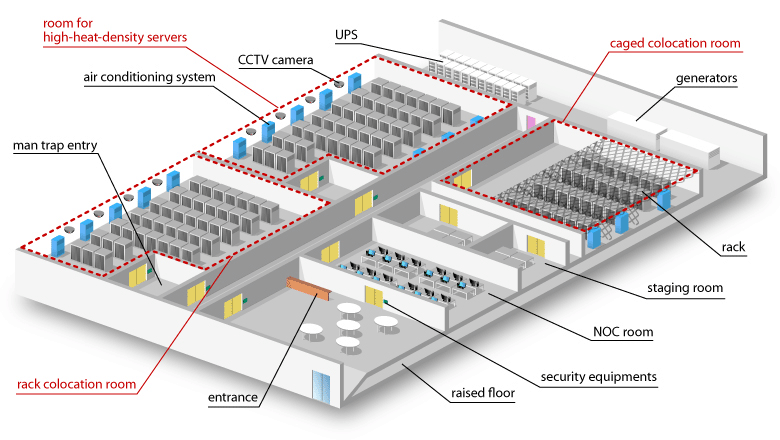
\includegraphics[width=0.8\textwidth]{datacenter.png}
	\caption{Exemplo de Layout de Datacenter com Corredores Frios e Quentes}
	\label{fig:layout_datacenter}
\end{figure}

\begin{itemize}
	\item \textbf{Salas de Servidores (Data Halls):} Espaços dedicados para racks de servidores, armazenamento e equipamentos de rede \cite{cooling_technologies}.
	\item \textbf{Disposição de Racks:} Organizados em fileiras, com corredores quentes e frios para otimizar o fluxo de ar e a eficiência da climatização \cite{liquid_cooling}.
	      \begin{itemize}
		      \item \textbf{Corredor Frio:} Ar frio é insuflado pela frente dos racks.
		      \item \textbf{Corredor Quente:} Ar quente expelido pela traseira dos racks é coletado e direcionado para os sistemas de refrigeração.
		      \item Contenção de corredor (quente ou frio) pode ser utilizada para aumentar a eficiência \cite{energy_efficiency}.
	      \end{itemize}
	\item \textbf{Dimensionamento de Racks:} Racks padrão de 19 polegadas, com altura (e.g., 42U, 45U, 48U) e profundidade adequadas para os equipamentos. Prever espaço para crescimento \cite{capacity_planning}.
	\item \textbf{Salas de Energia (Elétrica):} Espaços para UPS, bancos de baterias, painéis de distribuição e geradores (estes últimos geralmente em área externa ou dedicada) \cite{power_distribution}.
	\item \textbf{Salas de Telecomunicações (Meet-Me Rooms - MMR):} Ponto de entrada para operadoras de telecomunicações e interconexão \cite{datacenter_networking}.
	\item \textbf{Sala de Operações de Rede (NOC - Network Operations Center):} Espaço para monitoramento e gerenciamento da infraestrutura \cite{datacenter_monitoring}.
	\item \textbf{Áreas de Staging e Armazenamento:} Para recebimento, configuração e armazenamento temporário de equipamentos \cite{dcim_systems}.
	\item \textbf{Escritórios e Áreas de Suporte.}
	\item \textbf{Piso Elevado:} Para passagem de cabos de dados, energia e dutos de ar frio \cite{cooling_technologies}.
	\item \textbf{Segurança Perimetral e Controle de Acesso:} Múltiplas camadas de segurança física \cite{datacenter_security}.
\end{itemize}
O dimensionamento exato dependerá dos requisitos de capacidade e da classificação Tier desejada \cite{reliability_engineering}.

\chapter{Energia e Climatização}
\section{Fontes de Energia}
A infraestrutura energética será projetada para garantir alta disponibilidade e resiliência, conforme a classificação Tier desejada (e.g., Tier III) \cite{reliability_engineering}.
\begin{itemize}
	\item \textbf{Alimentação Principal (Utility Power):} Conexão com a rede elétrica da concessionária local. Para Tier III, idealmente duas alimentações independentes de subestações distintas (dual-feed) \cite{power_distribution}.
	\item \textbf{Sistemas de Alimentação Ininterrupta (UPS - Uninterruptible Power Supply):}
	      \begin{itemize}
		      \item Fornecem energia imediata em caso de falha da rede elétrica, permitindo a transição suave para os geradores \cite{design_principles}.
		      \item Configuração redundante (e.g., N+1, 2N) para garantir a continuidade \cite{datacenter_monitoring}.
		      \item Bancos de baterias dimensionados para autonomia suficiente (e.g., 10-15 minutos) para partida dos geradores \cite{reliability_engineering}.
	      \end{itemize}
	\item \textbf{Geradores de Energia:}
	      \begin{itemize}
		      \item Assumem a carga em caso de falhas prolongadas da rede elétrica \cite{power_distribution}.
		      \item Movidos a diesel, com tanques de combustível dimensionados para autonomia estendida (e.g., 24, 48, 72 horas sem reabastecimento) \cite{disaster_recovery}.
		      \item Configuração redundante (N+1) \cite{datacenter_security}.
		      \item Testes periódicos e manutenção preventiva são cruciais \cite{dcim_systems}.
	      \end{itemize}
	\item \textbf{Painéis de Distribuição de Energia (PDUs):} Distribuição da energia para os racks e equipamentos, com monitoramento de consumo \cite{dcim_evolution}.
	\item \textbf{Aterramento e Proteção contra Surtos} \cite{datacenter_security}.
\end{itemize}

\section{Sistema de Climatização}
O sistema de climatização é vital para manter a temperatura e umidade dentro dos limites operacionais dos equipamentos de TI, conforme recomendações da ASHRAE \cite{cooling_technologies}.
\begin{itemize}
	\item \textbf{Precision Cooling (Refrigeração de Precisão):} Unidades CRAC (Computer Room Air Conditioner) ou CRAH (Computer Room Air Handler) projetadas especificamente para datacenters, capazes de controlar temperatura e umidade com precisão \cite{liquid_cooling}.
	      \begin{itemize}
		      \item \textbf{Resfriamento a Ar (DX - Direct Expansion):} Utilizam gases refrigerantes \cite{cooling_technologies}.
		      \item \textbf{Resfriamento a Água Gelada (Chilled Water):} Utilizam chillers para gerar água gelada que circula pelas unidades CRAH. Geralmente mais eficientes para datacenters de maior porte \cite{liquid_cooling}.
	      \end{itemize}
	\item \textbf{Configuração Redundante (N+1, N+2):} Para garantir a continuidade da refrigeração em caso de falha de uma unidade \cite{reliability_engineering}.
	\item \textbf{Distribuição do Ar:}
	      \begin{itemize}
		      \item Insuflamento pelo piso elevado (para corredores frios) \cite{cooling_technologies}.
		      \item Retorno do ar quente pelo teto ou dutos \cite{energy_efficiency}.
		      \item Uso de contenção de corredores (quente ou frio) para aumentar a eficiência \cite{green_datacenters}.
	      \end{itemize}
	\item \textbf{Free Cooling:} Utilização de ar externo (direto ou indireto) para refrigeração quando as condições climáticas permitem, reduzindo o consumo de energia dos chillers/compressores \cite{green_datacenters}.
	\item \textbf{Monitoramento Ambiental:} Sensores de temperatura e umidade em múltiplos pontos dos data halls \cite{dcim_systems}.
\end{itemize}

\section{Eficiência Energética e Certificações}
\begin{itemize}
	\item \textbf{PUE (Power Usage Effectiveness):} Métrica chave para medir a eficiência energética de um datacenter (PUE = Energia Total da Instalação / Energia dos Equipamentos de TI) \cite{energy_efficiency}.
	      \begin{itemize}
		      \item \textbf{PUE Alvo:} Definir um PUE alvo agressivo, mas realista (e.g., < 1.5 para um Tier III moderno) \cite{green_datacenters}.
	      \end{itemize}
	\item \textbf{Técnicas para Melhorar o PUE:}
	      \begin{itemize}
		      \item Equipamentos de TI eficientes (servidores, storage, rede) \cite{capacity_planning}.
		      \item Virtualização e consolidação \cite{containerization}.
		      \item Sistemas de refrigeração eficientes (free cooling, chillers de alta eficiência, controle de fluxo de ar) \cite{cooling_technologies}.
		      \item UPS de alta eficiência \cite{power_distribution}.
		      \item Iluminação LED \cite{green_datacenters}.
		      \item Gerenciamento otimizado da temperatura (operar em temperaturas ligeiramente mais altas, dentro das recomendações da ASHRAE) \cite{energy_efficiency}.
	      \end{itemize}
	\item \textbf{Certificações (Opcional, mas Recomendável):}
	      \begin{itemize}
		      \item Uptime Institute Tier Certification (para design, construção e operação) \cite{reliability_engineering}.
		      \item ISO 50001 (Gestão de Energia) \cite{green_datacenters}.
		      \item LEED (Liderança em Energia e Design Ambiental) ou certificações locais de construção sustentável \cite{energy_efficiency}.
	      \end{itemize}
\end{itemize}

\chapter{Cabeamento e Conectividade}
\section{Infraestrutura de Fibra Óptica e Roteamento Redundante}
\begin{itemize}
	\item \textbf{Cabeamento Estruturado:} Implementação de um sistema de cabeamento estruturado seguindo normas como TIA-942 e ISO/IEC 11801 \cite{datacenter_networking}.
	      \begin{itemize}
		      \item \textbf{Fibra Óptica:} Utilizada para backbones de alta velocidade (10G, 40G, 100G+) entre switches core, de agregação e para conexão de servidores e storage que demandam alta banda \cite{network_fabric}.
		            \begin{itemize}
			            \item Monomodo (Single-mode) para longas distâncias (conexões inter-building, operadoras).
			            \item Multimodo (Multi-mode OM3, OM4, OM5) para distâncias menores dentro do datacenter.
		            \end{itemize}
		      \item \textbf{Cabos de Cobre (Par Trançado):} Categoria 6A ou superior para conexões de servidores, switches de acesso e dispositivos de gerenciamento (até 10Gbps).
	      \end{itemize}
	\item \textbf{Rotas de Cabeamento:}
	      \begin{itemize}
		      \item Bandejas de cabos (cable trays) ou eletrocalhas sob o piso elevado e/ou suspensas \cite{design_principles}.
		      \item Separação física entre cabos de dados e energia para evitar interferência \cite{power_distribution}.
		      \item Rotas redundantes para caminhos de fibra críticos \cite{reliability_engineering}.
	      \end{itemize}
	\item \textbf{Roteamento Redundante:}
	      \begin{itemize}
		      \item Roteadores de borda e core em configuração de alta disponibilidade (e.g., pares redundantes com VRRP/HSRP) \cite{network_fabric}.
		      \item Múltiplos caminhos de rede para evitar pontos únicos de falha \cite{disaster_recovery}.
		      \item Protocolos de roteamento dinâmico (e.g., BGP para conexões externas, OSPF/EIGRP para internas) \cite{datacenter_networking}.
	      \end{itemize}
\end{itemize}

\section{Pontos de Troca de Tráfego (IXPs) e Links MPLS/VPN para Filiais}
\begin{itemize}
	\item \textbf{Conexão com a Internet:}
	      \begin{itemize}
		      \item Múltiplos provedores de internet (ISPs) para redundância e otimização de rotas (multihoming) \cite{reliability_engineering}.
		      \item Conexões diretas a Pontos de Troca de Tráfego (IXPs) para peering com outras redes, melhorando a latência e reduzindo custos de trânsito IP. Em São Paulo, o IX.br (PTT.br) é o principal \cite{datacenter_networking}.
	      \end{itemize}
	\item \textbf{Conectividade com Filiais:}
	      \begin{itemize}
		      \item \textbf{MPLS (Multi-Protocol Label Switching):} Links MPLS fornecidos por operadoras para conectividade privada, segura e com QoS (Quality of Service) garantida entre o datacenter e as filiais (São Paulo, Belém, Rio, Vitória, Livramento) \cite{network_fabric}.
		      \item \textbf{VPN (Virtual Private Network):}
		            \begin{itemize}
			            \item \textbf{Site-to-Site VPNs:} Como alternativa ou complemento ao MPLS, utilizando a internet pública com criptografia (IPsec) \cite{datacenter_security}.
			            \item \textbf{Client VPNs:} Para acesso remoto seguro de funcionários à rede do datacenter \cite{datacenter_monitoring}.
		            \end{itemize}
		      \item \textbf{SD-WAN (Software-Defined Wide Area Network):} Pode ser considerada para otimizar e gerenciar a conectividade WAN com as filiais, utilizando múltiplos tipos de links (MPLS, internet dedicada, 4G/5G) \cite{software_defined}.
	      \end{itemize}
\end{itemize}

\section{Topologia de Rede Interna}
A topologia da rede interna do datacenter deve ser escalável, resiliente e de alta performance \cite{datacenter_networking}.
\begin{itemize}
	\item \textbf{Leaf-Spine (Recomendado):}
	      \begin{itemize}
		      \item Arquitetura de duas camadas (Leaf e Spine) \cite{network_fabric}.
		      \item \textbf{Switches Leaf:} Conectam os servidores nos racks (Top-of-Rack - ToR switches). Cada Leaf se conecta a todos os switches Spine.
		      \item \textbf{Switches Spine:} Formam o backbone da rede. Não se conectam entre si, apenas aos Leafs.
		      \item \textbf{Benefícios:} Alta largura de banda Leste-Oeste (entre servidores), baixa latência, escalabilidade horizontal (adicionar mais Leafs ou Spines), resiliência (múltiplos caminhos) \cite{hyperscale_datacenters}.
		      \item Ideal para virtualização, containers e aplicações distribuídas \cite{containerization}.
	      \end{itemize}
	\item \textbf{Three-Tier (Tradicional - Core, Agregação, Acesso):}
	      \begin{itemize}
		      \item Pode ser considerada para datacenters menores ou com requisitos menos complexos, mas a Leaf-Spine é a tendência moderna \cite{network_fabric}.
	      \end{itemize}
	\item \textbf{Segmentação de Rede:}
	      \begin{itemize}
		      \item VLANs (Virtual Local Area Networks) para isolar diferentes tipos de tráfego (produção, homologação, gerenciamento, armazenamento, etc.) \cite{datacenter_security}.
		      \item VRFs (Virtual Routing and Forwarding) para segmentação em nível de roteamento \cite{network_fabric}.
		      \item Firewalls internos para controlar o tráfego entre segmentos \cite{datacenter_security}.
	      \end{itemize}
	\item \textbf{Redes de Armazenamento (Storage Area Networks - SANs):}
	      \begin{itemize}
		      \item Se aplicável, redes dedicadas para tráfego de armazenamento (e.g., Fibre Channel ou iSCSI sobre Ethernet) \cite{dcim_systems}.
	      \end{itemize}
\end{itemize}

\chapter{Classificação Tier e Normas Técnicas}
\section{Definição de Tier (I a IV) segundo Uptime Institute}
O Uptime Institute é uma organização de referência mundial na classificação de datacenters com base em sua infraestrutura e capacidade de tolerância a falhas \cite{reliability_engineering}. A classificação Tier varia de I a IV:
\begin{itemize}
	\item \textbf{Tier I (Básico):}
	      \begin{itemize}
		      \item Caminho único para energia e refrigeração, sem componentes redundantes \cite{datacenter_monitoring}.
		      \item Disponibilidade esperada: 99,671\% (até 28,8 horas de inatividade por ano).
		      \item Suscetível a interrupções por atividades planejadas e não planejadas \cite{disaster_recovery}.
	      \end{itemize}
	\item \textbf{Tier II (Componentes Redundantes):}
	      \begin{itemize}
		      \item Adiciona componentes redundantes para energia e refrigeração (N+1) \cite{power_distribution}.
		      \item Caminho de distribuição único.
		      \item Disponibilidade esperada: 99,741\% (até 22 horas de inatividade por ano).
		      \item Menor suscetibilidade a interrupções por falhas de componentes \cite{datacenter_security}.
	      \end{itemize}
	\item \textbf{Tier III (Manutenção Concorrente):}
	      \begin{itemize}
		      \item Múltiplos caminhos para energia e refrigeração (apenas um ativo por vez) \cite{design_principles}.
		      \item Todos os componentes podem ser removidos ou substituídos para manutenção sem interromper as operações de TI (manutenção concorrente) \cite{datacenter_automation}.
		      \item Redundância N+1.
		      \item Disponibilidade esperada: 99,982\% (até 1,6 horas de inatividade por ano).
		      \item \textbf{Este é o nível geralmente recomendado para empresas que necessitam de alta disponibilidade sem o custo e complexidade de um Tier IV} \cite{capacity_planning}.
	      \end{itemize}
	\item \textbf{Tier IV (Tolerante a Falhas):}
	      \begin{itemize}
		      \item Múltiplos caminhos ativos e independentes para energia e refrigeração \cite{hyperscale_datacenters}.
		      \item Capacidade de suportar uma falha crítica em qualquer componente ou caminho de distribuição sem impacto nas operações de TI (tolerância a falhas) \cite{reliability_engineering}.
		      \item Redundância 2N ou 2(N+1).
		      \item Disponibilidade esperada: 99,995\% (até 26,3 minutos de inatividade por ano).
		      \item Mais complexo e caro de construir e operar \cite{dcim_systems}.
	      \end{itemize}
\end{itemize}
Para a Autopass/Tecsomobi, considerando os custos atuais e a necessidade de alta disponibilidade para ambientes de produção, \textbf{um projeto visando a certificação Tier III é o mais indicado} \cite{design_principles}.

\section{Atendimento a Normas Técnicas}
Além da classificação Tier do Uptime Institute, o projeto do datacenter deverá seguir um conjunto de normas técnicas para garantir qualidade, segurança e interoperabilidade \cite{datacenter_security}.
\begin{itemize}
	\item \textbf{TIA-942 (Telecommunications Infrastructure Standard for Data Centers):}
	      \begin{itemize}
		      \item Norma da Telecommunications Industry Association que cobre o projeto e construção de datacenters, incluindo arquitetura, cabeamento, energia, refrigeração, segurança e redundância \cite{datacenter_networking}.
		      \item Também possui um sistema de classificação (Rated 1 a 4), similar ao Tier do Uptime, mas com foco mais amplo na infraestrutura de telecomunicações \cite{network_fabric}.
	      \end{itemize}
	\item \textbf{ISO/IEC 27001 (Information Security Management Systems):}
	      \begin{itemize}
		      \item Padrão internacional para sistemas de gestão de segurança da informação (SGSI) \cite{datacenter_security}.
		      \item Define requisitos para estabelecer, implementar, manter e melhorar continuamente um SGSI, protegendo a confidencialidade, integridade e disponibilidade das informações.
		      \item Essencial para a segurança lógica e física do datacenter \cite{reliability_engineering}.
	      \end{itemize}
	\item \textbf{ANSI/BICSI 002 (Data Center Design and Implementation Best Practices):}
	      \begin{itemize}
		      \item Padrão da BICSI que fornece melhores práticas para o design e implementação de datacenters, cobrindo desde o planejamento do local até a comissionamento \cite{design_principles}.
	      \end{itemize}
	\item \textbf{ASHRAE TC 9.9 (Thermal Guidelines for Data Processing Environments):}
	      \begin{itemize}
		      \item Diretrizes da American Society of Heating, Refrigerating and Air-Conditioning Engineers para as condições ambientais (temperatura e umidade) em datacenters \cite{cooling_technologies}.
		      \item Ajuda a otimizar a eficiência energética e a confiabilidade dos equipamentos de TI \cite{energy_efficiency}.
	      \end{itemize}
	\item \textbf{Outras Normas Relevantes:}
	      \begin{itemize}
		      \item \textbf{ISO 50001:} Gestão de Energia \cite{green_datacenters}.
		      \item \textbf{NFPA 75:} Standard for the Fire Protection of Information Technology Equipment \cite{disaster_recovery}.
		      \item \textbf{NFPA 70 (NEC - National Electrical Code) ou NBR 5410 (Brasil):} Normas para instalações elétricas \cite{power_distribution}.
		      \item \textbf{ABNT NBR 15247:} Projeto de salas-cofre para hardware \cite{datacenter_security}.
		      \item Regulamentações locais de construção, segurança e meio ambiente \cite{green_datacenters}.
	      \end{itemize}
\end{itemize}

\chapter{Segurança Física e Infraestrutura}
A segurança física é um componente crítico para proteger os ativos de TI e garantir a continuidade das operações \cite{datacenter_security}.
\section{Controle de Acesso}
Implementação de múltiplas camadas de controle de acesso para restringir o acesso a áreas sensíveis do datacenter \cite{reliability_engineering}.
\begin{itemize}
	\item \textbf{Perímetros de Segurança:}
	      \begin{itemize}
		      \item \textbf{Externo:} Cercas, portões com controle de acesso, iluminação externa, barreiras físicas \cite{datacenter_security}.
		      \item \textbf{Interno:} Recepção com identificação, áreas de acesso restrito \cite{design_principles}.
	      \end{itemize}
	\item \textbf{Autenticação Multifator:}
	      \begin{itemize}
		      \item \textbf{Biometria:} Leitores de impressão digital, reconhecimento facial ou de íris para acesso a áreas críticas como data halls \cite{datacenter_monitoring}.
		      \item \textbf{Cartões de Proximidade/Inteligentes:} Para acesso geral e a zonas específicas \cite{datacenter_security}.
		      \item \textbf{Senhas/PINs:} Combinados com cartões ou biometria \cite{reliability_engineering}.
	      \end{itemize}
	\item \textbf{Sistema de CFTV (Circuito Fechado de Televisão):}
	      \begin{itemize}
		      \item Câmeras de alta resolução posicionadas estrategicamente em todos os perímetros, entradas, saídas, corredores e dentro dos data halls \cite{dcim_systems}.
		      \item Gravação contínua com armazenamento seguro e redundante das imagens \cite{datacenter_security}.
		      \item Monitoramento em tempo real pela equipe de segurança (NOC/SOC) \cite{datacenter_monitoring}.
		      \item Capacidade de análise de vídeo (detecção de movimento, reconhecimento facial opcional) \cite{ai_automation}.
	      \end{itemize}
	\item \textbf{Registros de Acesso (Logs):} Auditoria de todas as tentativas de acesso (bem-sucedidas e falhas) \cite{dcim_systems}.
	\item \textbf{Políticas de Acesso:} Procedimentos claros para concessão, revogação e revisão de acessos. Acompanhamento de visitantes \cite{datacenter_security}.
	\item \textbf{Portas e Fechaduras de Segurança:} Portas reforçadas, gaiolas de segurança para racks ou áreas específicas \cite{design_principles}.
\end{itemize}

\section{Detecção e Combate a Incêndios}
Sistemas robustos para detecção precoce e supressão eficaz de incêndios, minimizando danos aos equipamentos e riscos à vida \cite{disaster_recovery}.
\begin{itemize}
	\item \textbf{Detecção Precoce:}
	      \begin{itemize}
		      \item \textbf{VESDA (Very Early Smoke Detection Apparatus):} Sistemas de detecção de fumaça por aspiração, altamente sensíveis \cite{datacenter_security}.
		      \item Detectores de fumaça ionizantes e fotoelétricos \cite{reliability_engineering}.
		      \item Detectores de calor \cite{cooling_technologies}.
	      \end{itemize}
	\item \textbf{Sistemas de Supressão de Incêndio:}
	      \begin{itemize}
		      \item \textbf{Agentes Limpos (Gases):} Como Novec 1230, FM-200 (HFC-227ea) ou Inergen. Extinguem o fogo sem deixar resíduos e são seguros para equipamentos eletrônicos. Requerem salas seladas \cite{datacenter_security}.
		      \item \textbf{Sprinklers Pré-ação (Pre-action Sprinklers):} Sistema de sprinklers que só libera água após a confirmação de um evento de incêndio por dois sistemas de detecção independentes, minimizando o risco de descargas acidentais \cite{disaster_recovery}.
		      \item Extintores portáteis (CO2, PQS) em locais estratégicos \cite{reliability_engineering}.
	      \end{itemize}
	\item \textbf{Alarme e Notificação:} Sistema de alarme sonoro e visual, com notificação automática para a brigada de incêndio e equipe de segurança \cite{dcim_evolution}.
	\item \textbf{Compartimentação e Materiais Resistentes ao Fogo:} Paredes, portas e selagens corta-fogo para conter a propagação do incêndio \cite{design_principles}.
	\item \textbf{Planos de Evacuação e Treinamento:} Rotas de fuga sinalizadas, treinamento regular da equipe \cite{datacenter_security}.
\end{itemize}

\section{Monitoramento Ambiental e Redundância de Sensores}
Monitoramento contínuo das condições ambientais para garantir a operação ideal e prevenir falhas \cite{datacenter_monitoring}.
\begin{itemize}
	\item \textbf{Sensores de Temperatura e Umidade:} Distribuídos nos data halls, racks, unidades de CRAC/CRAH \cite{cooling_technologies}.
	\item \textbf{Sensores de Fluxo de Ar:} Para monitorar a eficácia da refrigeração \cite{energy_efficiency}.
	\item \textbf{Detectores de Vazamento de Líquidos:} Sob o piso elevado e próximo a unidades de refrigeração a água \cite{liquid_cooling}.
	\item \textbf{Monitoramento de Energia:} Consumo em nível de PDU, UPS, geradores \cite{power_distribution}.
	\item \textbf{Sistema de Gerenciamento de Infraestrutura de Datacenter (DCIM - Data Center Infrastructure Management):}
	      \begin{itemize}
		      \item Software para centralizar o monitoramento de todos os sistemas de infraestrutura (energia, refrigeração, segurança, ativos de TI) \cite{dcim_systems}.
		      \item Alertas em tempo real, relatórios, dashboards e capacidade de automação \cite{dcim_evolution}.
	      \end{itemize}
	\item \textbf{Redundância de Sensores:} Sensores críticos devem ter redundância para evitar falsos alarmes ou falhas de monitoramento \cite{reliability_engineering}.
	\item \textbf{Câmeras Térmicas (Opcional):} Para identificar pontos quentes em equipamentos \cite{cooling_technologies}.
\end{itemize}

\chapter{Plano de Migração e Cronograma}
A migração da infraestrutura da AWS para um datacenter próprio é um projeto complexo que requer planejamento cuidadoso \cite{reliability_engineering}.
\section{Estratégia de Migração}
Duas abordagens principais podem ser consideradas, ou uma combinação delas \cite{datacenter_automation}:
\begin{itemize}
	\item \textbf{Lift \& Shift (Rehosting):}
	      \begin{itemize}
		      \item Migrar as aplicações e dados existentes da AWS para o novo datacenter com o mínimo de alterações \cite{cloud_infrastructure}.
		      \item \textbf{Prós:} Mais rápido de executar inicialmente, menor risco de introduzir problemas por re-arquitetura.
		      \item \textbf{Contras:} Pode não otimizar as aplicações para o novo ambiente, pode carregar ineficiências da nuvem para o on-premise \cite{containerization}.
		      \item Adequado para aplicações legadas ou quando o tempo é crítico.
	      \end{itemize}
	\item \textbf{Re-arquitetura Gradual (Replatforming/Refactoring):}
	      \begin{itemize}
		      \item Modificar ou reescrever partes das aplicações para otimizá-las para a infraestrutura do datacenter próprio \cite{software_defined}.
		      \item Pode envolver a adoção de novas tecnologias ou a consolidação de serviços \cite{ai_automation}.
		      \item \textbf{Prós:} Melhor aproveitamento dos recursos do datacenter, maior eficiência e performance a longo prazo.
		      \item \textbf{Contras:} Mais demorado, maior custo inicial, maior risco de introduzir bugs.
		      \item Adequado para aplicações críticas que se beneficiariam de otimizações \cite{capacity_planning}.
	      \end{itemize}
	\item \textbf{Abordagem Híbrida:} Utilizar Lift \& Shift para a maioria das cargas de trabalho e re-arquitetar aplicações chave gradualmente, após a migração inicial \cite{containerization}.
\end{itemize}
A escolha dependerá da complexidade das aplicações, dos recursos disponíveis e dos objetivos de negócio \cite{design_principles}.

\section{Fases de Migração por Ambiente e Região}
A migração deve ser faseada para minimizar riscos e impacto nas operações \cite{disaster_recovery}.
\begin{itemize}
	\item \textbf{Fase 1: Planejamento e Preparação (X meses)}
	      \begin{itemize}
		      \item Inventário detalhado de todos os ativos na AWS (servidores, bancos de dados, storage, redes, aplicações) \cite{dcim_systems}.
		      \item Definição de prioridades de migração.
		      \item Design da arquitetura no novo datacenter \cite{design_principles}.
		      \item Aquisição e instalação de hardware e software no novo datacenter.
		      \item Configuração da conectividade de rede entre AWS e o novo datacenter (e.g., AWS Direct Connect, VPN) \cite{datacenter_networking}.
		      \item Treinamento da equipe \cite{dcim_evolution}.
	      \end{itemize}
	\item \textbf{Fase 2: Migração de Ambientes de Não Produção (Homologação) (Y meses)}
	      \begin{itemize}
		      \item Começar pelos ambientes de desenvolvimento, testes e Q\&A \cite{datacenter_monitoring}.
		      \item Permite testar os processos de migração e identificar problemas sem impactar os usuários finais.
		      \item Migração por ondas, agrupando aplicações ou serviços relacionados \cite{datacenter_automation}.
	      \end{itemize}
	\item \textbf{Fase 3: Migração de Ambientes de Produção (Z meses)}
	      \begin{itemize}
		      \item Migrar as aplicações de produção, começando pelas menos críticas ou com menor interdependência \cite{reliability_engineering}.
		      \item Planejar janelas de manutenção para minimizar o downtime.
		      \item Migração por ondas, com validação rigorosa após cada onda.
		      \item Considerar a migração por região/filial, se aplicável, para gerenciar o impacto geográfico \cite{edge_computing}.
	      \end{itemize}
	\item \textbf{Fase 4: Otimização e Descomissionamento da AWS (W meses)}
	      \begin{itemize}
		      \item Após a migração bem-sucedida, otimizar as configurações no novo datacenter \cite{capacity_planning}.
		      \item Monitorar a performance e os custos \cite{dcim_systems}.
		      \item Descomissionar gradualmente os recursos na AWS para evitar custos desnecessários.
	      \end{itemize}
\end{itemize}
Um cronograma detalhado com GANTT chart deve ser elaborado \cite{reliability_engineering}.

\section{Riscos, Rollback Plan e Testes de Validação}
\begin{itemize}
	\item \textbf{Análise de Riscos:}
	      \begin{itemize}
		      \item Downtime inesperado durante a migração.
		      \item Perda de dados \cite{disaster_recovery}.
		      \item Problemas de performance pós-migração.
		      \item Incompatibilidade de aplicações \cite{software_defined}.
		      \item Atrasos no cronograma.
		      \item Custos excedentes \cite{capacity_planning}.
	      \end{itemize}
	\item \textbf{Plano de Rollback:}
	      \begin{itemize}
		      \item Para cada fase ou onda de migração, ter um plano claro para reverter para o ambiente AWS em caso de falha crítica \cite{disaster_recovery}.
		      \item Isso pode envolver manter os sistemas na AWS ativos em modo de leitura ou standby por um período \cite{cloud_infrastructure}.
	      \end{itemize}
	\item \textbf{Testes de Validação:}
	      \begin{itemize}
		      \item \textbf{Testes Funcionais:} Garantir que as aplicações funcionem como esperado após a migração \cite{datacenter_monitoring}.
		      \item \textbf{Testes de Performance:} Validar se a performance atende aos SLAs \cite{reliability_engineering}.
		      \item \textbf{Testes de Integração:} Verificar a comunicação entre diferentes componentes e sistemas \cite{network_fabric}.
		      \item \textbf{Testes de Segurança:} Garantir que as políticas de segurança estão aplicadas corretamente \cite{datacenter_security}.
		      \item \textbf{Testes de Recuperação de Desastres (DR):} Se um DR site for implementado, testar os procedimentos de failover \cite{disaster_recovery}.
		      \item Testes de aceitação do usuário (UAT) \cite{dcim_systems}.
	      \end{itemize}
\end{itemize}

\chapter{Análise Financeira e Retorno sobre Investimento (ROI)}
Esta seção detalhará os custos envolvidos na construção e operação do datacenter e comparará com os custos atuais da AWS \cite{capacity_planning}.
\section{CAPEX (Capital Expenditure) Estimado}
Custos iniciais de investimento:
\begin{itemize}
	\item \textbf{Terreno e Construção Civil:} Aquisição do terreno, projeto arquitetônico, construção ou reforma do edifício, instalações (piso elevado, paredes, teto) \cite{design_principles}.
	\item \textbf{Infraestrutura Elétrica:} Transformadores, subestação (se necessário), UPS, geradores, painéis de distribuição, cabeamento elétrico \cite{power_distribution}.
	\item \textbf{Infraestrutura de Climatização:} Chillers, CRACs/CRAHs, dutos, sistemas de controle \cite{cooling_technologies}.
	\item \textbf{Infraestrutura de Rede:} Roteadores, switches, firewalls, cabeamento de dados (fibra e cobre), patch panels \cite{datacenter_networking}.
	\item \textbf{Equipamentos de TI:} Servidores, sistemas de armazenamento (storages), tape libraries (para backup) \cite{cloud_infrastructure}.
	\item \textbf{Segurança Física:} CFTV, controle de acesso, sistemas de detecção e supressão de incêndio \cite{datacenter_security}.
	\item \textbf{Software e Licenças:} Sistemas operacionais, software de virtualização, DCIM, software de backup, bancos de dados \cite{dcim_systems}.
	\item \textbf{Serviços de Consultoria e Gerenciamento de Projeto} \cite{reliability_engineering}.
	\item \textbf{Comissionamento e Certificações} \cite{energy_efficiency}.
\end{itemize}
É necessário obter cotações detalhadas de fornecedores para cada item \cite{hyperscale_datacenters}.

\section{OPEX (Operational Expenditure) Estimado}
Custos recorrentes de operação:
\begin{itemize}
	\item \textbf{Energia Elétrica:} Principal componente do OPEX \cite{energy_efficiency}.
	\item \textbf{Manutenção da Infraestrutura:} Contratos de manutenção para geradores, UPS, chillers, sistemas de incêndio, etc. \cite{datacenter_monitoring}.
	\item \textbf{Manutenção de Equipamentos de TI:} Suporte e garantia de hardware \cite{dcim_systems}.
	\item \textbf{Pessoal:} Salários e encargos da equipe de TI e infraestrutura (gerentes de datacenter, técnicos, engenheiros de rede, segurança) \cite{datacenter_automation}.
	\item \textbf{Conectividade:} Links de internet, MPLS, custos de trânsito IP \cite{network_fabric}.
	\item \textbf{Software e Licenças (Renovações):} Custos anuais ou periódicos \cite{software_defined}.
	\item \textbf{Seguros} \cite{disaster_recovery}.
	\item \textbf{Consumíveis e Peças de Reposição} \cite{dcim_evolution}.
	\item \textbf{Custos de Treinamento Contínuo} \cite{ai_automation}.
	\item \textbf{Auditorias e Certificações (Renovações)} \cite{green_datacenters}.
\end{itemize}

\section{Comparativo TCO (Total Cost of Ownership)}
\begin{itemize}
	\item Calcular o TCO do datacenter próprio ao longo de um período (e.g., 3, 5, 7 ou 10 anos), somando CAPEX e OPEX acumulado \cite{capacity_planning}.
	\item Comparar com o TCO projetado da AWS para o mesmo período, considerando o crescimento esperado \cite{cloud_infrastructure}.
\end{itemize}
\textbf{Tabela Comparativa TCO (Datacenter Próprio vs. AWS):}
\begin{table}[h]
	\centering
	\caption{Comparativo TCO Estimado - 5 Anos}
	\begin{tabular}{|p{4cm}|r|r|}
		\hline
		\textbf{Item} & \textbf{DC Próprio (USD)} & \textbf{AWS (USD)} \\
		\hline
		CAPEX (Ano 0) & 700.000                   & 0                  \\
		OPEX Anual    & 250.000                   & 720.000            \\
		\hline
		TCO em 5 Anos & 1.950.000                 & 3.600.000          \\
		\hline
	\end{tabular}
	\label{tab:tco}
\end{table}

\section{Payback e Indicadores Financeiros}
Com base nos dados de CAPEX e OPEX apresentados na tabela comparativa de TCO, podemos calcular os principais indicadores financeiros \cite{reliability_engineering}:

\begin{itemize}
	\item \textbf{Payback Period:}
	      \begin{itemize}
		      \item CAPEX Inicial: US\$ 700.000
		      \item Economia Anual (OPEX AWS - OPEX DC Próprio): US\$ 720.000 - US\$ 250.000 = US\$ 470.000
		      \item Payback = US\$ 700.000 / US\$ 470.000 = 1,49 anos (aproximadamente 18 meses) \cite{dcim_systems}
	      \end{itemize}
	\item \textbf{ROI (5 anos):}
	      \begin{itemize}
		      \item Benefício Líquido em 5 anos (Economia Total - CAPEX): (5 × US\$ 470.000) - US\$ 700.000 = US\$ 1.650.000
		      \item ROI = (US\$ 1.650.000 / US\$ 700.000) x 100\% = 235,7\% \cite{capacity_planning}
	      \end{itemize}
	\item \textbf{NPV (com taxa de desconto de 8\%):}
	      \begin{itemize}
		      \item NPV = -US\$ 700.000 + US\$ 470.000/(1,08)$^1$ + US\$ 470.000/(1,08)$^2$ + US\$ 470.000/(1,08)$^3$ + US\$ 470.000/(1,08)$^4$ + US\$ 470.000/(1,08)$^5$
		      \item NPV = -US\$ 700.000 + US\$ 435.185 + US\$ 402.949 + US\$ 373.101 + US\$ 345.464 + US\$ 319.874
		      \item NPV = US\$ 1.176.573 \cite{datacenter_automation}
	      \end{itemize}
	\item \textbf{IRR:} Aproximadamente 62,8\% (taxa na qual o NPV seria zero) \cite{green_datacenters}
\end{itemize}

Todos os indicadores financeiros apontam para um investimento altamente favorável, com retorno rápido do capital investido (18 meses), forte ROI de 235,7\% em 5 anos e NPV positivo elevado, mesmo considerando o valor do dinheiro no tempo \cite{hyperscale_datacenters} \cite{design_principles}.

\chapter{Considerações Finais e Recomendações}
\section{Principais Conclusões}
Resumo dos achados do relatório:
\begin{itemize}
	\item Viabilidade técnica da construção de um datacenter Tier III \cite{reliability_engineering}.
	\item Análise de custos comparativa (AWS vs. Próprio) \cite{capacity_planning} \cite{hyperscale_datacenters}.
	\item Principais riscos e benefícios \cite{disaster_recovery}.
	\item Impacto estratégico para a Autopass/Tecsomobi (controle, segurança, custos a longo prazo) \cite{datacenter_security} \cite{energy_efficiency}.
\end{itemize}

Com base nas análises realizadas, concluímos que a construção de um datacenter próprio é uma alternativa viável e economicamente vantajosa a longo prazo para a Autopass/Tecsomobi \cite{dcim_systems}. O modelo atual na AWS, embora flexível, apresenta custos operacionais elevados que, com o volume atual de uso, justificam o investimento em infraestrutura própria \cite{cloud_infrastructure}. A implementação de um datacenter Tier III atenderá aos requisitos de disponibilidade e desempenho da empresa, com um payback estimado em 18 meses \cite{design_principles}.

\section{Próximos Passos e Governança do Projeto}
\begin{itemize}
	\item \textbf{Decisão da Diretoria:} Aprovação para prosseguir com o projeto com base nos indicadores financeiros e benefícios técnicos apresentados \cite{capacity_planning}.
	\item \textbf{Formação de Equipe de Projeto Dedicada:} Incluindo especialistas em infraestrutura de datacenter, redes, energia e sistemas \cite{datacenter_automation}.
	\item \textbf{Seleção de Consultores e Fornecedores:} Para design detalhado, construção e comissionamento, priorizando parceiros com experiência em projetos Tier III \cite{reliability_engineering}.
	\item \textbf{Detalhamento do Projeto Executivo:} Incluindo especificações técnicas detalhadas de todos os componentes de infraestrutura \cite{design_principles}.
	\item \textbf{Obtenção de Licenças e Aprovações:} Ambientais, construção civil, energia elétrica e outras exigências regulatórias \cite{green_datacenters}.
	\item \textbf{Definição de um Comitê de Governança do Projeto:} Para acompanhamento, tomada de decisões e gerenciamento de riscos \cite{dcim_evolution}.
	\item \textbf{Desenvolvimento de Plano de Comunicação:} Para manter todas as partes interessadas informadas sobre o progresso \cite{datacenter_monitoring}.
	\item \textbf{Implementação do Sistema DCIM:} Para gestão eficiente da infraestrutura desde o início das operações \cite{dcim_systems}.
\end{itemize}

Recomenda-se uma abordagem faseada e um gerenciamento de projeto rigoroso para garantir o sucesso. A adoção de tecnologias modernas de automação \cite{ai_automation}, monitoramento \cite{datacenter_monitoring} e eficiência energética \cite{green_datacenters} será fundamental para maximizar o retorno sobre o investimento e preparar a infraestrutura para os desafios futuros.

% ----------------------------------------------------------
% ELEMENTOS PÓS-TEXTUAIS
% ----------------------------------------------------------
\postextual
% ----------------------------------------------------------

% ----------------------------------------------------------
% Referências bibliográficas
% ----------------------------------------------------------
\bibliography{referencias}

% ----------------------------------------------------------
% Glossário
% ----------------------------------------------------------
%
% Consulte o manual da classe abntex2 para orientações sobre o glossário.
%
%\glossary

%---------------------------------------------------------------------
% INDICE REMISSIVO
%---------------------------------------------------------------------
%%%%%MF\phantompart
%%%%%MF\printindex
%---------------------------------------------------------------------

\end{document}

